La figura \ref{fig:gantt_inicial} muestra el diagrama de Gantt con la planificación inicial del proyecto.  La planificación inicial se ha realizado basándose en la Estructura de Desglose del Trabajo detallada en el apartado anterior.  A la Estructura de Desglose de Trabajo se han añadido las tareas de gestión del proyecto y los hitos necesarios para ir desarrollando el sistema.\\

A pesar de no figurar en el diagrama Gantt, cabe destacar que una vez por semana se realiza una reunión de seguimiento del proyecto por parte del equipo de desarrollo.  El objetivo de estas reuniones es informar a todo el equipo del avance del proyecto y tratar los posibles problemas y cambios que vayan surgiendo durante el desarrollo.

\begin{figure}[h]
	\centering
	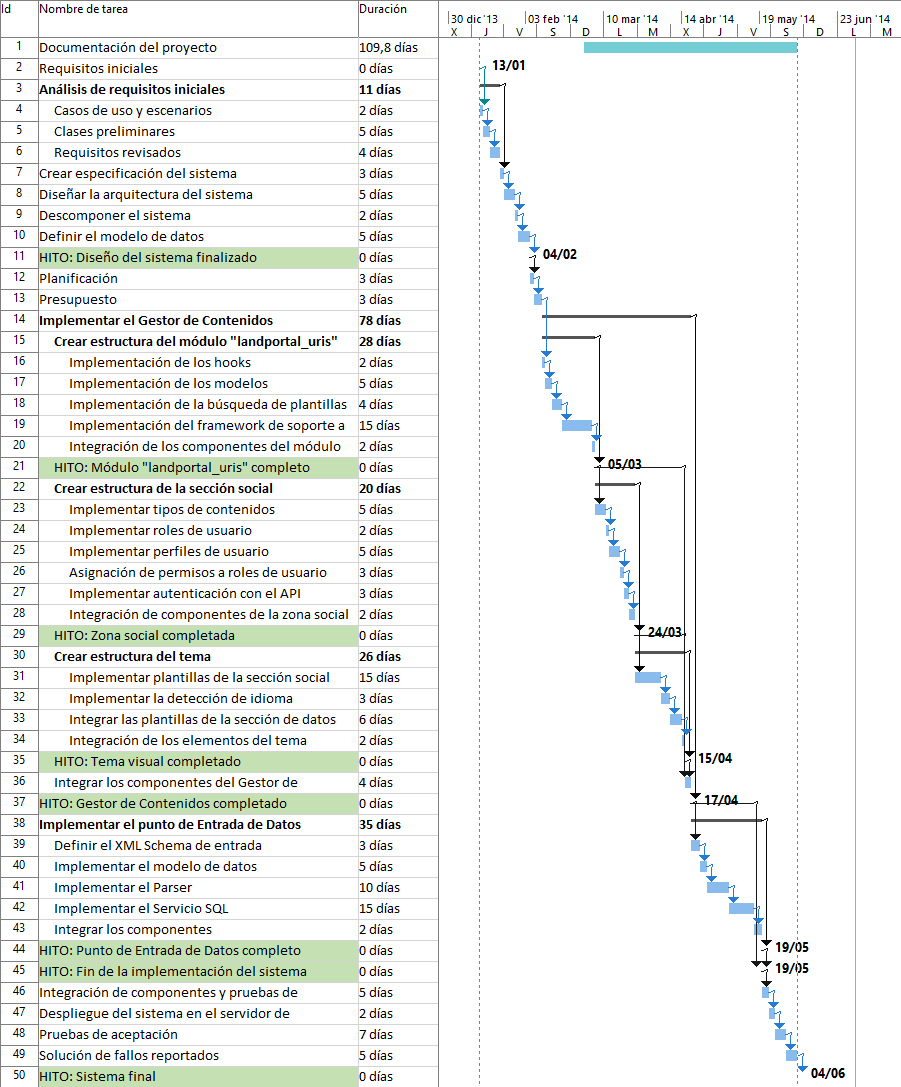
\includegraphics[width=\textwidth]{planificacion/inicial}
	\caption{Diagrama de Gantt con la planificación inicial del proyecto}
	\label{fig:gantt_inicial}
\end{figure}